\subsection{Architecture logicielle}

L'architecture de notre bibliothèque se constitue des deux package que sont \texttt{Detector} et \texttt{Filter}.

Le package \texttt{Detector} contient l'interface des méthodes de détection et reconnaissance de forme ainsi que leurs implémentation.
Le package \texttt{Filter} contient les filtres pour le prétraitement ainsi que la détection de nouveauté.


\begin{center}
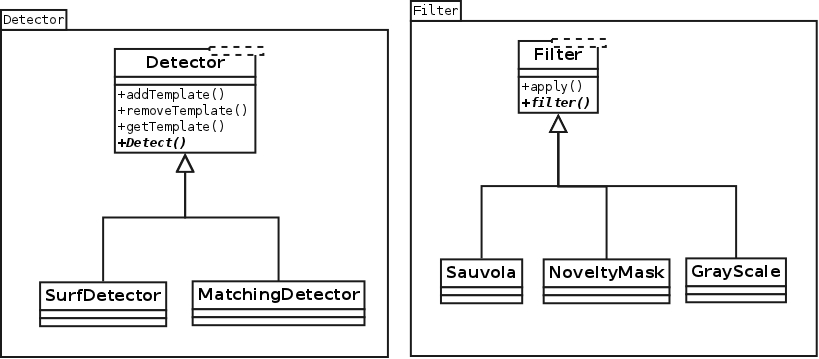
\includegraphics[width=\textwidth]{Archi/Architecture.png}
\end{center}

\paragraph{Package \texttt{Filter}\\}
Le prétraitement des images réside essentiellement en l'application de filtres. Afin de simplifier ces application nous avons défini une interface commune à tous les filtres. 

Dans le but d'unifier le comportement des filtres nous utiliserons le patron de conception "patron de méthode" qui permet de définir la méthode \texttt{apply} qui permet d'appliquer le filtre sur l'image. 
L'interface des filtre devient donc une classe abstraire dans laquelle, seul la méthode \texttt{filter} reste à implémenter, elle contiendra le traitement réel du filtre.

On peut remarquer que certain filtres, comme la conversion d'une image couleur en image niveau de gris, n'ont pas de paramètre particulier et de ce fait une seule instance doit être créer, les autre ne faisant que consommer inutilement la mémoire. L'utilisation du patron de conception "singleton" semble utile.

Toujours dans le but d'unifier l'utilisation des filtres, nous avons mis en place une fabrique de filtre, qui permet également d'assurer l'unicité de certains de ceux-ci.

\subsection{Pré-traitement} %penser à retoucher les sections.
Prétraitement : 
Nos images sont bruités  


Filtre passe bas, flou gaussien ...   
et 
augmentation de contraste...

sont des outils que nous avons utilisé pendant le projet   


étude du filtre de Weiner qui permet de flouter les zones homogéne et de réhausser les contrastes 


Avant de commencer la détection de nouveautés ou de forme nous devons segmenter notre image afin de détecter les objets sur l'image.

Etant donné le type de support, un document avec des symboles noirs sur fond blanc, nous avons focaliser notre travail sur la binarisation.

La binarisation à pour but de ségmenter l'image en 2 classes, le fond et l'image.
Il existe différentes techniques pour binariser une image.

Nous avons dans un premier temps étudié la binarisation par seuillage global, on choisit la classe du pixel à partir d'un seuil.

\begin{equation}
	\forall i,j \in \mathbf{M*N} \quad I(i,j)=
	\left\lbrace
	\begin{array}{ccc}
		1 &\mbox{si}& f(i,j) > S,\\
		0 &\mbox{sinon}&
	\end{array}\right.
\end{equation}

%%Avec : 
%%\begin{description}
%%  \item[ $N × M$] nombre de colonnes et de lignes de l’image ;
%%  \item[$I$] image binarisée ;
%%  \item[$S$] seuil de binarisation.
%%  \item[$f$] valeur fonction de l’image d’origine ;\ldots
%%  
%\end{description}

Le probléme est que l'on utilise des documents dégradés ( mauvaise ilumination et papier marqué) donc bien souvent il n'existe pas de seuil global.
'''''''Cf image'''''''''' 


Ensuite nous avons étudié la detection de contour car un dessin est une accumulation de trait.
Nous avons donc appliqué le filtre de Sobel et Canny à nos images.

Filtre de Sobel

Filtre de canny 



Les résultats étaient bien sur èfficace sur les traits fin mais moins bon dans les zones coloriées.
Toutefois il est possible d'obtenir, en y combinant des filtres morphologiques, les zones dans lesquelles il y a un objet.



L'étude de ,qui compare les différents algorithmes de binarisation emet un classement des meilleurs algorithmes pour les images dégradés.
La methode de kittler se basant sur le clustering ... nous avons abandonné cette méthode car les résultats obtenus étaient insuffisants.

et les méthodes par seuillage local, son principe est d’utiliser une étude localisée autour du pixel pour déterminer quel seuil utiliser. Pour réaliser cette étude locale, les techniques utilisent une fenêtre d’étude centrée sur le pixel à étudier. Cette fenêtre peut avoir différentes tailles, de nombreuses méthodes on été proposé bernsten, Niblack , Sauvola.

Sauvola est indiqué comme obtenant les meilleurs résultats

\begin{equation}
	S(i,j) = \mu(i,j) + \kappa.((\sigma(i,j)/R)-1))
\end{equation}

Avec :
- S(i, j) : seuil à appliquer pour le point i, j ;\\
- $\sigma(i, j)$ : valeur de l’écart type dans une fenêtre centré en i, j de taille $N * M$ ;\\
- $\mu(i, j)$ : valeur moyenne des niveaux de gris dans la même fenêtre ;\\
- $\kappa$ : constante fixée le plus généralement à 0, 2 ;\\
- R : constante permettant d'ajuster la dynamique de l'ecart type, géneralement 128.
- N et M appartenant à N.\\

La méthode de Sauvola calcule le seuil de binarisation en fonction de la moyenne et de l'ectart type des pixels ajuster par la constante R , le raport entre les deux est défini par la constante $\kappa$.
Sauvola conseille un $\kappa \in \left[ 0.2 ;0.5 \right[$, mais ce type de paramétre est fixé pour binariser des textes, or nos documents sont des dessins effectué au crayons a papier et peuvent avoir des trait trés fins.
dans son article  , fixe $\kappa$ à 0.05, ce qui augmente l'influence de l'ecart type et permet d'obtenir de meilleurs résultats, notament lorsqu'il y a un faible contraste comme dans notre cas.   

La taille de la fenêtre est fixé en fonction de la taille de l'image, nous ne prenons pas la même taille de fenetre pour l'image en haute résolution que pour le flux vidéo en basse résolution.

Optimisation.

Les images integrales sont une représentation sous la forme d'une image, de même taille que l'image d'origine, qui en chacun de ses points contient la somme des pixels situés au dessus et à gauche de ce point. Plus formellement, l'image intégrale ii est définie à partir de l'image i par : 

\begin{equation}
	%ii(x,y) = \sum \liminf{\underset{x' \leq x}{y' \leq y }} i(x',y')
	ii(x,y) = \sum_{x' \leq x  \atop y' \leq y } i(x',y')
\end{equation}







résumé des differentes techniques 


Seuillage global

detection de contour + filtre morphologique 
     
Seuillage local Opencv moyenne et gaussian

seuillage locale Sauvola


\subsection{Traitement}
\subsubsection{Détection des évolutions d'un dessin}
Un premier objectif du projet était d'extraire les moments clés de la réalisation d'un dessin.

\paragraph{Pré-traitement\vspace{0.5cm} \\}
La capture des images étant faite en haute qualité, l'étape de pré-traitement n'a pas une grande influence sur les résultats obtenus. Seul une correction de couleur (balance des blancs) est réalisée afin de corriger le changement de coloration générale de l'image acquise. On pourrait penser que cette correction pourrait être effectuée sur la camera directement, ce qui y est généralement fait, mais le processus de réalisation d'un dessin peut être long. De ce fait, la coloration due à l'éclairage de la scène peut varier\footnote{Cette dérive d'éclairage ne s'observe pas dans un environnement contrôlé, tels qu'un studio}. Dans la plupart de cas, cette correction doit être effectuée sur chaque image acquise.

\paragraph{Extraction des nouveautés\vspace{0.5cm}\\}
Une fois cette petite étape de pré-traitement effectuée nous pouvons commencer à extraire les nouveautés.

Dans un premier temps, nous avons effectué de simples différences entre les images mais cela n'a pas été concluant. En effet, l'acquisition de deux images à deux instants différents induisent des différences de positions du dessin ainsi que de légères variations d'éclairage. Ainsi, comme on le voit sur les images ci-dessous, le résultat obtenu n'est pas celui attendu. 

\begin{center}
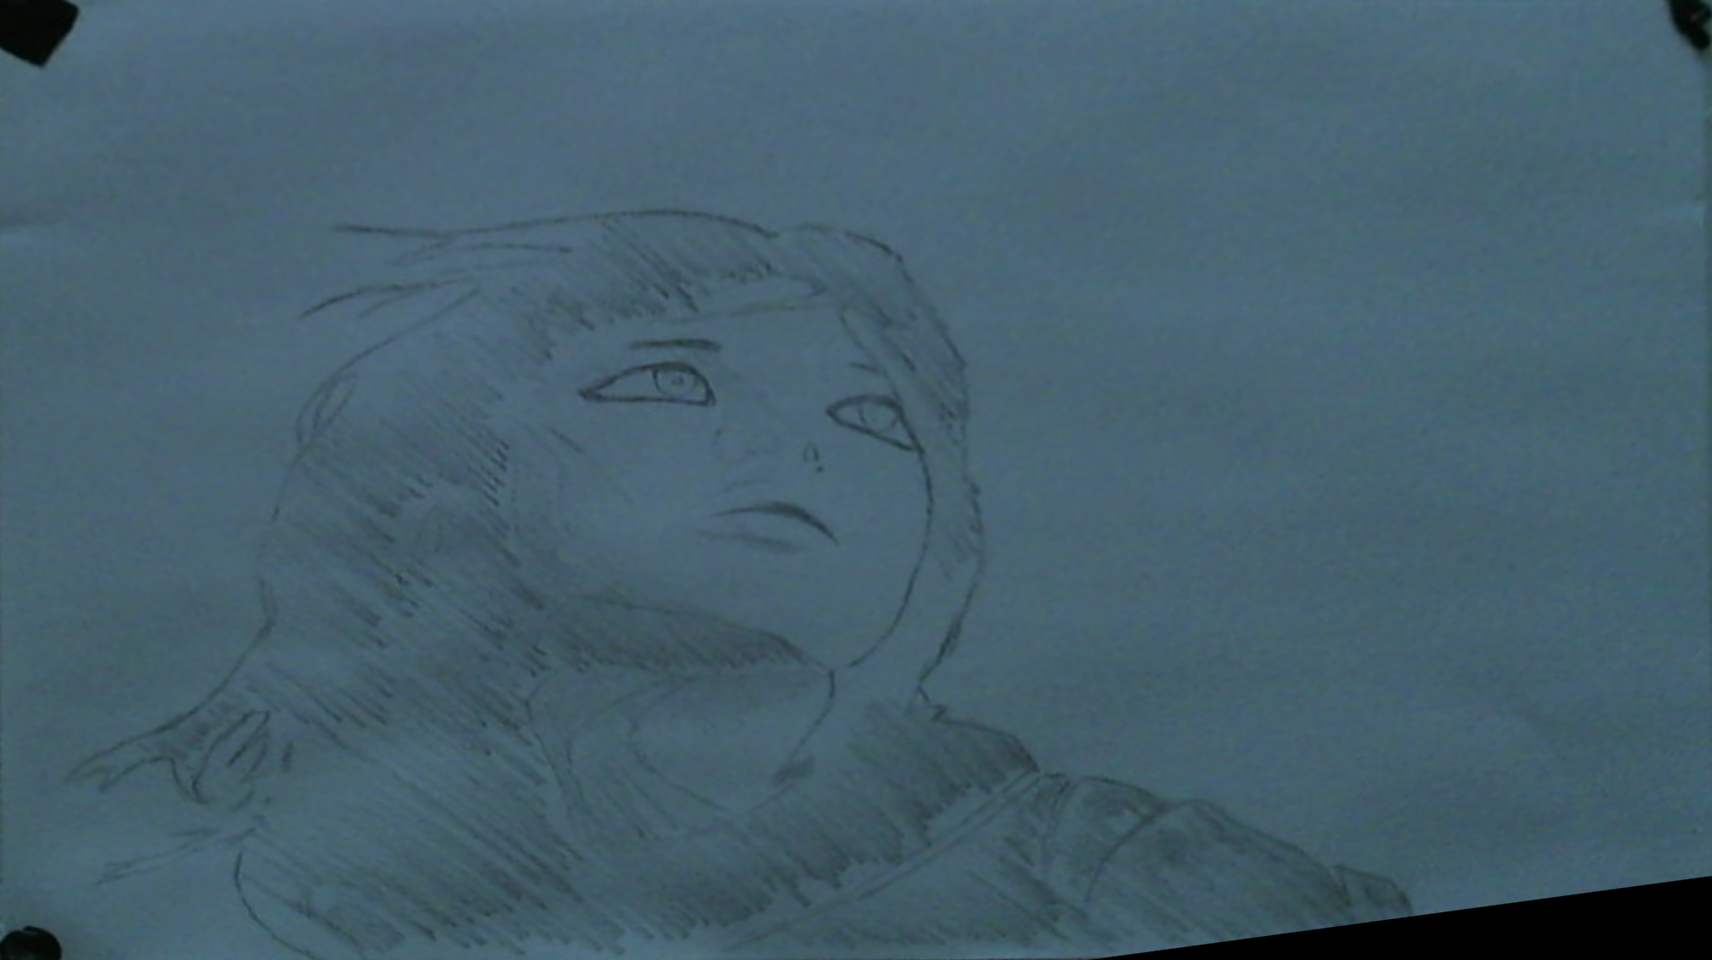
\includegraphics[width=6.5cm]{images/capImage1-7.png}
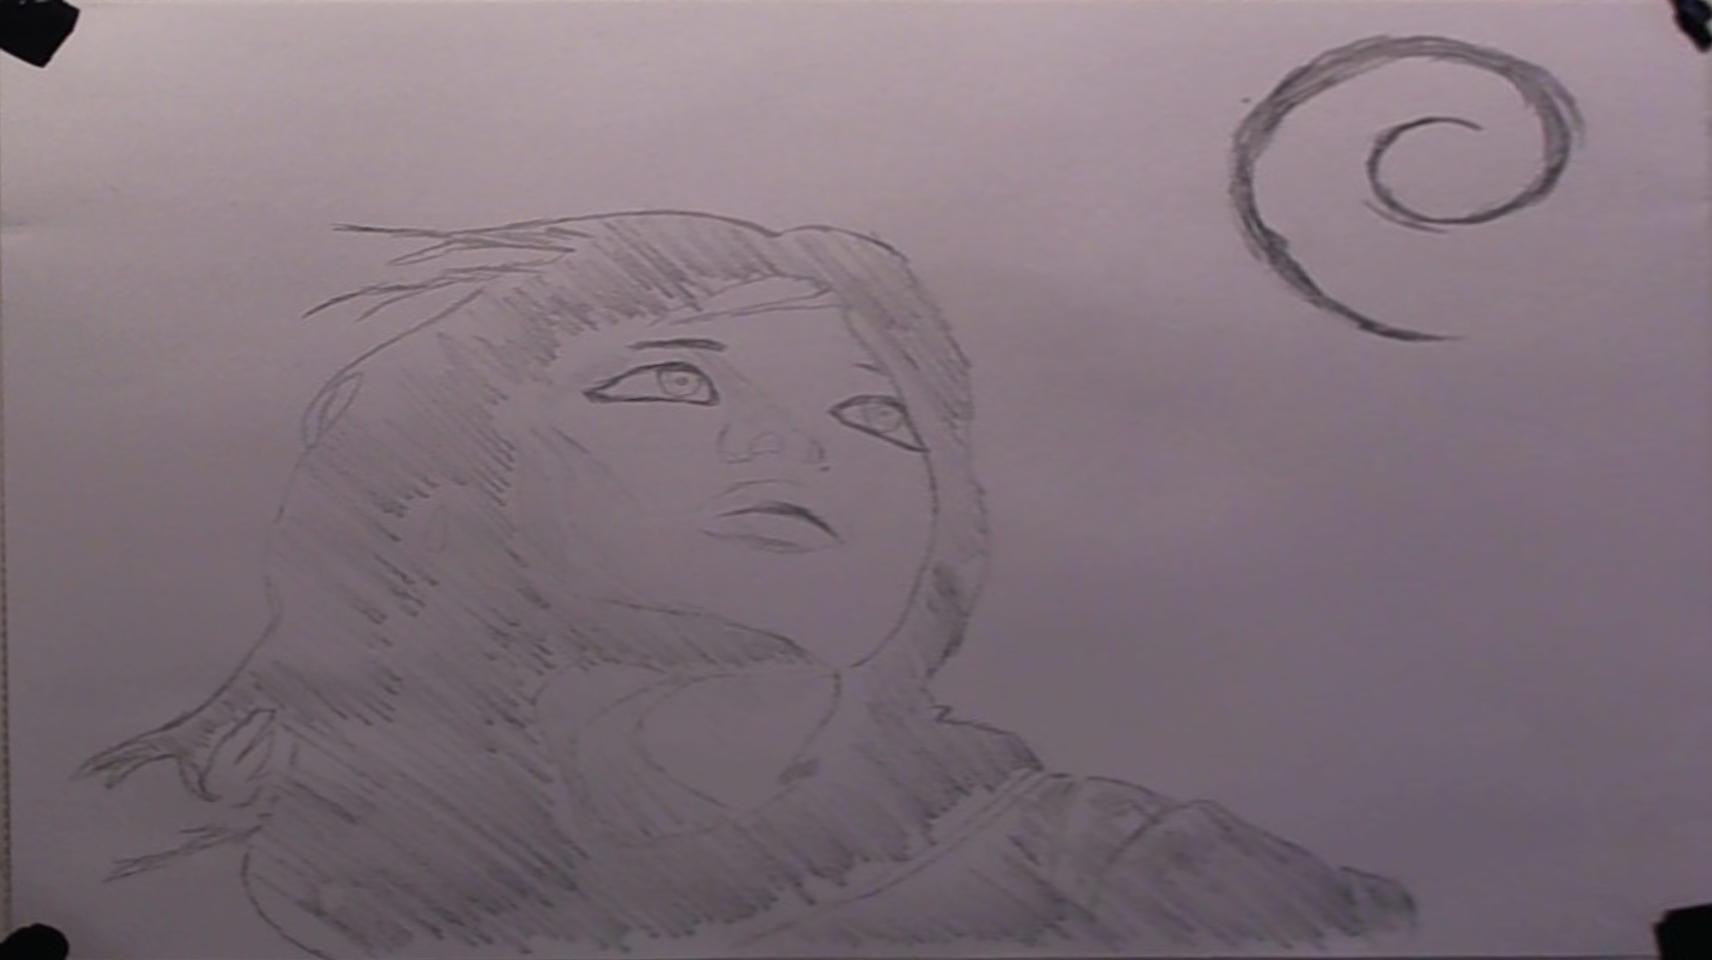
\includegraphics[width=6.5cm]{images/capImage1-9.png}
\hfill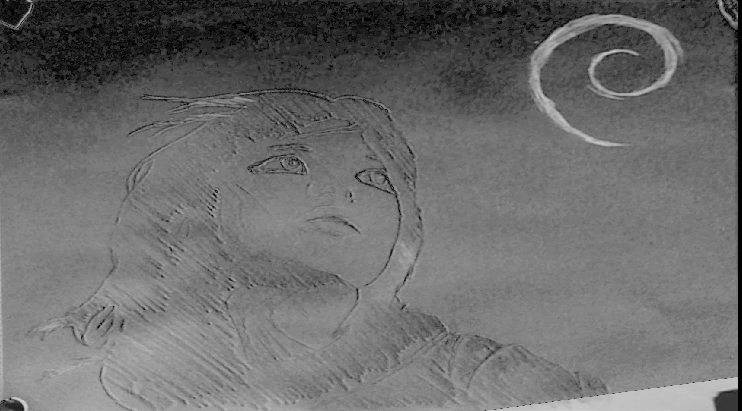
\includegraphics[width=6.5cm]{images/simpleDiff.png}\newline
\captionof{figure}{Image du bas : résultat de la simple différence en les images du haut}
\end{center}

Nous avons donc, dans un second temps, extrait un masque de nouveauté, c'est-à-dire, une image binaire dans laquelle les zones ayant changées sont blanches, toutes les autres étant noires. Ce masque nous permet de récupérer, dans l'image originale, uniquement les nouveautés du dessin.


\begin{center}
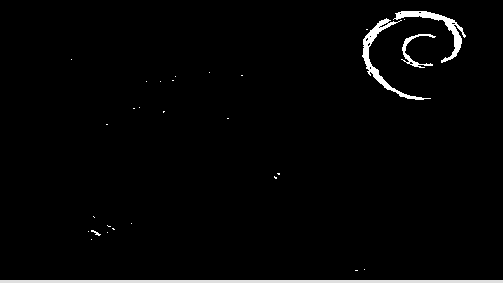
\includegraphics[width=8cm]{images/masqueDiff.png}\newline
\captionof{figure}{Masque de différence obtenu à partir des deux images précédentes}
\end{center}

Pour obtenir ce masque, nous binarisons les deux images à partir desquelles nous voulons extraire les nouveautés. Puis nous faisons la différence des deux images obtenues, les images étant binarisées, on obtient directement un masque de nouveauté.

\subsubsection{Reconnaissance de formes dessinées}

Afin de reconnaître des formes simples dans une vidéo, nous avons mis en place un système de détecteur.\\

Nous avons implémenté deux détecteurs différents. Le premier s'appuie sur du template matching pour reconnaître une forme. Le second utilise les descripteurs SURF.\\

Pour faire ainsi, nous avons mis en place une classe abstraite \texttt{Detector} qui présente les fonctions de base d'un détecteur, à savoir ajouter, récupérer ou supprimer un template, et définit la fonction permettant de lancer la détection.
Chacun de nos détecteurs (\texttt{MatchingDetector et SurfDetector} doit donc implémenter cette fonction de détection.

\paragraph{Template matching\vspace{0.5cm}\\}

Notre premier détecteur est le \texttt{MatchingDetector}, qui utilise l'algorithme de template matching.\\

L'algorithme de template matching consiste à faire glisser un template sur la surface de l'image, et de calculer un coefficient de "corrélation" entre le template et la zone qu'il recouvre.\\

Pour effectuer cette procédure, nous parcourons la liste des templates du détecteur. Pour chacun de ces templates, nous avons utilisé la fonction \texttt{cvMatchTemplate} d'OpenCV pour calculer une image de corrélation entre le template et l'image tirée de la vidéo, qui montre les endroits où le template a le plus correspondu à l'image. Après normalisation, nous parcourons cette image pour récupérer le minimum (ou maximum suivant la méthode passée en paramètre à \texttt{cvMatchTemplate}), ce minimum/maximum est l'endroit de meilleur matching. Nous stockons alors le quadruplet $(x,y,w,h)$ avec :
\begin{description}
\item[x,y] Les coordonnées du point de meilleur matching correspondant au coin supérieur gauche de la zone rectangulaire représentant l'objet détecté.
\item[w,h] Les dimensions du template, correspondant aux dimensions de la zone rectangulaire représentant l'objet détecté.\\
\end{description}

Une fois la position du meilleur matching récupérée, nous retirons de l'image source la zone rectangulaire décrite par le quadruplet $(x,y,w,h)$. Cette étape permet d'éviter que deux templates trop proches détectent le même objet alors que deux objets sont valides (exemple : Sur un dessin, deux bonhommes sont dessinés. Avec deux templates de bonhomme, il est possible que les deux matchings trouvent comme meilleur résultat le premier bonhomme et ne détectent pas le second. Notre étape de suppression permet de faire en sorte qu'une fois que le premier matching a détecté le premier bonhomme, celui-ci n'est plus pris en compte pour les détections des autres templates. On augmente ainsi les chances de détecter tous les objets de l'image.)\\

Une fois tous les templates parcourus, nous retournons l'ensemble des quadruplets $(x,y,w,h)$ correspondant aux détections.\\

Un des défauts de notre \texttt{MatchingDetector} est que le retour de\\ \texttt{cvMatchTemplate} ne nous permet pas de calculer un seuil de confiance pour accepter ou rejeter le résultat du matching. On peut récupérer l'endroit où le template a le plus correspondu à l'image, mais on ne sait pas si il a matché à 99\% où à 10\%.\\

Ce défaut, couplé à la normalisation du résultat de \texttt{cvMatchTemplate} (première tentative, infructueuse, de déterminer un seuil de confiance) entraîne un faux positif lorsque le template ne matche pas un des objets de l'image.\\ Le problème est double : pour le moment, nous avons un template = un résultat. On a donc forcément des faux positifs lorsque le nombre de templates d'un type d'objet dépasse le nombre d'objets de ce type du dessin, ou quand le template ne matche pas à un des objets du dessin. Nous avons également des faux négatifs, donc des objets qui ne sont pas détectés, lorsque le nombre de templates d'un type d'objet est inférieur au nombre d'objets de ce type dans le dessin.\\

Une solution au problème serait d'arriver à calculer un indice de confiance du matching. Si cet indice de confiance ne dépasse pas un seuil à définir, on ne prend pas en compte le résultat du matching pour ce template.\\

Cette solution permet de boucler sur un template jusqu'à ce que l'indice de confiance calculé ne passe plus le seuil. Cela permet d'avoir un template par type d'objet, et non un template = un résultat positif comme à présent. Avec peu de templates de bonhomme, on pourrait détecter un grand nombre de bonshommes dans le dessin. On réduirait ainsi le problème de faux négatifs lorsque le nombre de templates d'un type d'objet est inférieur au nombre d'objets de ce type. Et comme on ne prend pas en compte les matchings qui ne passent pas le seuil, on réduit également le nombre de faux positifs.\\


\paragraph{SURF : Speeded Up Robust Features\\}
L'algorithme SURF consiste à calculer des descripteurs sur les templates ainsi que sur l'image. Une fois ces descripteurs calculés, on en fait quelque chose.

"SURF[11] : Speeded Up Robust Features" is a high-performance scale and rotation-invariant interest point detector / descriptor claimed to approximate or even outperform previously proposed schemes with respect to repeatability, distinctiveness, and robustness. SURF relies on integral images for image convolutions to reduce computation time, builds on the strengths of the leading existing detectors and descriptors (using a fast Hessian matrix-based measure for the detector and a distribution-based descriptor). It describes a distribution of Haar wavelet responses within the interest point neighbourhood. Integral images are used for speed and only 64 dimensions are used reducing the time for feature computation and matching. The indexing step is based on the sign of the Laplacian, which increases the matching speed and the robustness of the descriptor.


